\documentclass[11pt]{article}
\usepackage[T1]{fontenc}
\usepackage[utf8]{inputenc}
\usepackage{lmodern}
\usepackage[margin=0.85in]{geometry}
\usepackage{microtype}
\usepackage{amsmath,amssymb}
\usepackage{booktabs}
\usepackage{array}
\usepackage{enumitem}
\usepackage{xcolor}
\usepackage{tikz}
\usepackage{hyperref}
\usepackage[numbers,sort&compress]{natbib}
\usepackage{titlesec}
\hypersetup{colorlinks=true,linkcolor=blue!60!black,citecolor=blue!60!black,urlcolor=blue!60!black}
\setlist[itemize]{topsep=3pt,itemsep=2pt,leftmargin=1.4em}
\setlist[enumerate]{topsep=3pt,itemsep=2pt,leftmargin=1.6em}
\titleformat{\section}{\large\bfseries}{\thesection}{0.6em}{}
\titleformat{\subsection}{\normalsize\bfseries}{\thesubsection}{0.6em}{}
\titleformat{\subsubsection}{\normalsize\itshape}{\thesubsubsection}{0.6em}{}

\newcommand{\term}[1]{\textbf{#1}}
\newcommand{\flow}{flow control}

\title{Evolution and State of the Art in Flow Control for Network-on-Chip Interconnects\\\large With Emphasis on Ring and Hierarchical-Ring Topologies}
\author{Prepared by Ditto}
\date{\today}

\begin{document}
\maketitle

\begin{abstract}
This report surveys the evolution of NoC flow control for multicore processors, from store-and-forward and virtual cut-through to wormhole, virtual-channel, credit-based, elastic-buffer, and bufferless/deflection designs. The emphasis is ring-based NoCs, including simple rings, hierarchical rings, and the HiRD design (``Design and Evaluation of Hierarchical Rings with Deflection Routing'') by Ausavarungnirun et al. The main conclusion is that rings remain attractive when layout regularity, low router cost, coherent traffic ordering, and moderate core counts dominate, but their flow-control choices are tightly coupled to injection fairness, ejection priority, and congestion isolation. For larger and less locality-friendly systems, the state of the art usually shifts toward meshes or hierarchical/high-radix designs using credit-based wormhole flow control, a small number of virtual channels, protocol-level virtual networks, and sometimes adaptive or bypass mechanisms. Bufferless/deflection flow control is the most ring-relevant research alternative because it converts backpressure into extra path length, but it must be engineered carefully to avoid livelock, starvation, and pathological latency.
\end{abstract}

\section{Executive takeaways}

\begin{enumerate}
  \item \term{The industrial default is conservative.} Publicly documented NoCs in multicore processors and coherent fabrics usually emphasize lossless packet/flit transport, local backpressure or credits, separated traffic classes, and simple deadlock rules. This is less glamorous than some research proposals, but easier to time, verify, and integrate with coherence.
  \item \term{Rings are not obsolete, but they are niche-optimal.} A ring has tiny routers, natural layout regularity, and simple arbitration. The cost is poor bisection bandwidth and distance growth. Hierarchical rings try to preserve ring simplicity locally while reducing global traversal distance.
  \item \term{Ring flow control has three canonical families.} Slot/token/circuit-style rings avoid buffer competition by scheduling slots; credit or ready/valid rings apply backpressure when downstream buffers fill; deflection/bufferless rings avoid stopping by misrouting or re-circulating packets.
  \item \term{HiRD's core idea is to use deflection as the ring analogue of buffering.} Hierarchical Rings with Deflection Routing (HiRD) connects small local rings through a global ring and uses deflection at local/global interfaces and destinations to avoid expensive buffering and global backpressure \cite{Ausavarungnirun2014HiRD}. This makes the router simple and buffer-light, but shifts the burden to fairness, livelock freedom, and injection/ejection policy.
  \item \term{For non-ring NoCs, virtual channels remain the workhorse.} VC flow control, introduced by Dally \cite{Dally1990VC,Dally1992VC}, is still the cleanest way to decouple traffic classes, reduce head-of-line blocking, provide escape resources for adaptive routing, and break coherence-protocol dependency cycles.
  \item \term{The research frontier is conditional, not universal.} Express virtual channels, SMART, elastic buffers, and bufferless/minimally buffered designs each optimize a different bottleneck: hop latency, buffer area/leakage, or low-load latency. None dominates all workloads and physical design constraints.
\end{enumerate}

\section{What exactly is ``flow control'' in a NoC?}

In a NoC, \flow{} decides when a sender may inject or forward a flit/packet into a downstream resource. It is distinct from routing, which chooses the path, and arbitration, which chooses among contenders for the same output. In practice the three are coupled: a router can only route through outputs whose downstream buffers, slots, or credits are available.

The central trade-off is simple: \emph{buffer when blocked, stop the sender, reserve capacity ahead of time, or send the packet somewhere else}. Most NoC flow-control mechanisms are combinations of these four responses.

\begin{itemize}
  \item \term{Store-and-forward}: buffer the whole packet at every hop. Simple, but too buffer-heavy and high-latency for many on-chip fabrics.
  \item \term{Virtual cut-through}: forward as soon as the next router can accept the whole packet; otherwise buffer the packet \cite{Kermani1979VirtualCutThrough}.
  \item \term{Wormhole}: split packets into flits; a header flit reserves route state and following flits pipeline through. This drastically reduces buffer capacity but creates channel-holding dependencies that can deadlock \cite{NiMcKinley1993,DallyTowles2004Book}.
  \item \term{Credit-based flow control}: upstream maintains a count of free downstream buffer slots. Sending consumes a credit; freeing a slot returns a credit. It is precise and lossless, but credit round-trip latency determines how much buffering is needed.
  \item \term{Virtual-channel flow control}: multiplex multiple logical queues over one physical link. VCs reduce head-of-line blocking and are the standard tool for deadlock avoidance, adaptive routing escape paths, and coherence traffic-class isolation \cite{Dally1990VC,Dally1992VC}.
  \item \term{Elastic/bufferless/deflection}: reduce or eliminate input buffers. Elastic-buffer NoCs store flits in link pipeline registers \cite{Michelogiannakis2009Elastic}; bufferless deflection routes a contending flit to a non-minimal output rather than waiting \cite{Moscibroda2009,Fallin2011CHIPPER}.
\end{itemize}

\section{Historical evolution}

\subsection{Before NoCs: switching and deadlock foundations}

Virtual cut-through, wormhole routing, and deadlock theory predate the NoC term. Dally and Seitz's channel-dependency graph formalized when a routing function can deadlock: a cycle in the channel dependency graph is dangerous because packets can each hold one channel while waiting for the next \cite{DallySeitz1987DeadlockFree}. Wormhole routing made this especially important because a blocked packet may hold buffers and links across multiple hops.

Dally's virtual-channel work then introduced a practical hardware mechanism to split one physical channel into multiple logical channels \cite{Dally1990VC,Dally1992VC}. This matters because a physical wire can remain busy even when one logical flow is blocked. It also lets a designer impose acyclic resource ordering without duplicating physical links.

\subsection{NoC era: packets, not global wires}

The early-2000s NoC argument was that global buses and ad hoc wiring do not scale with core count and SoC complexity. Dally and Towles' ``route packets, not wires'' paper and Benini/de Micheli's NoC paradigm paper framed on-chip interconnects as packet-switched networks with explicit topology, routing, flow control, and router microarchitecture \cite{DallyTowles2001,BeniniDeMicheli2002}.

The classic wormhole VC router pipeline has input buffering, route computation, VC allocation, switch allocation, switch traversal, and link traversal. Peh and Dally modeled these delays and proposed speculation to reduce pipeline cost \cite{PehDally2001}; Mullins et al. further optimized low-latency VC routers \cite{Mullins2004}. This is still the baseline mental model for a mesh NoC router.

\subsection{Mid-2000s onward: reduce hop count or remove buffers}

Two lines of work attacked NoC cost from opposite directions:

\begin{itemize}
  \item \term{Bypass and high-radix designs} reduce the number or cost of router stops. Express virtual channels bypass intermediate routers \cite{Kumar2007EVC}; flattened butterfly reduces diameter by using higher-radix routers \cite{Kim2007Flattened}; SMART tries to traverse several routers in one cycle when setup arbitration succeeds \cite{Krishna2013SMART}.
  \item \term{Buffer reduction designs} reduce storage and allocator complexity. Elastic buffers place storage in links \cite{Michelogiannakis2009Elastic}. Bufferless and minimally buffered deflection routers remove most input buffering and route losers to alternate outputs \cite{Moscibroda2009,Michelogiannakis2010Bufferless,Fallin2011CHIPPER,Fallin2012MinBD}.
\end{itemize}

The practical lesson is that the best mechanism depends on whether the bottleneck is hop latency, buffer area/leakage, energy per bit, saturation throughput, or verification complexity. Modern industrial fabrics generally choose robust combinations rather than maximal academic cleverness.

\section{Ring-based NoCs}

\subsection{Why rings are attractive}

A ring router can be extremely small: one or two transit directions, injection/ejection ports, and local arbitration. Rings also provide a naturally pipelined layout around cores, last-level-cache slices, memory controllers, or coherent agents. That is why rings appeared in commercial designs such as Intel client/server processors and IBM Cell's Element Interconnect Bus (EIB) \cite{Kanter2010Sandy,Ainsworth2006Cell}.

The downside is equally fundamental. A single unidirectional ring has bisection bandwidth proportional to link width, not node count. Mean distance grows with ring size. A bidirectional ring helps latency and bandwidth but adds direction choice, ordering concerns, and possible deadlock if packets can hold resources while turning or changing rings. Hierarchical rings reduce distance by using local rings for nearby traffic and a global ring for inter-cluster traffic \cite{Ravindran1998HierRing,Das2009Hier,Ausavarungnirun2014HiRD}.

\subsection{Canonical ring flow-control styles}

\subsubsection{Slot, token, and circuit-style rings}

In a slotted ring, each cycle or pipeline slot is either empty or carries a packet/flit. A node injects only when it sees an empty slot or owns a token/credit. IBM Cell's EIB is a useful industry example: public analyses describe four data rings plus a command bus, pipelined circuit-switched transfers, and end-to-end command credits before elements issue command-bus requests \cite{Ainsworth2006Cell}. Slot/token designs have excellent simplicity and bounded arbitration, but under bursty traffic unused slots and head-of-line effects can hurt utilization.

\subsubsection{Credit/backpressure rings}

A ring can also use local ready/valid or credit-based backpressure. If the next ring stop has no space, upstream stops forwarding. This is lossless and simple for short rings, but in a cycle it can create global stalls unless the design preserves empty buffers or orders resources carefully. Bubble flow control is the classic solution: allow injection only if enough empty buffer slots remain to guarantee at least one ``bubble'' circulates, breaking cyclic wait conditions \cite{Carrion1997Bubble}. In a wormhole ring or torus, bubble rules are a cheap alternative to adding many VCs, though they reduce usable buffering at high load.

\subsubsection{Virtual-channel rings}

VCs can break a ring's cyclic dependency by splitting traffic into ordered classes or by using escape resources. This is common in torus and mesh theory and also relevant to rings that support bidirectional movement, multiple message classes, or coherence request/response interactions. The cost is that even a simple ring stop becomes a VC router with per-VC buffers, credits, and arbitration.

\subsubsection{Deflection and bufferless rings}

Deflection replaces ``wait'' with ``go somewhere else.'' In a ring, the simplest deflection is re-circulation: if a packet cannot eject or transfer to another ring, it continues around and tries later. In a hierarchical ring, a packet can also miss a bridge opportunity and keep circulating on the local or global ring. This avoids backpressure and input buffering but consumes extra bandwidth and can inflate tail latency.

The deflection family is attractive for rings because the output choice space is small and router critical paths can be kept short. However, correctness depends on four policies: ejection priority, injection throttling, age/fairness, and rules for transfer between local/global rings. Without those, a packet can be repeatedly bypassed by younger traffic, creating starvation or severe latency outliers.

\begin{figure}[t]
\centering
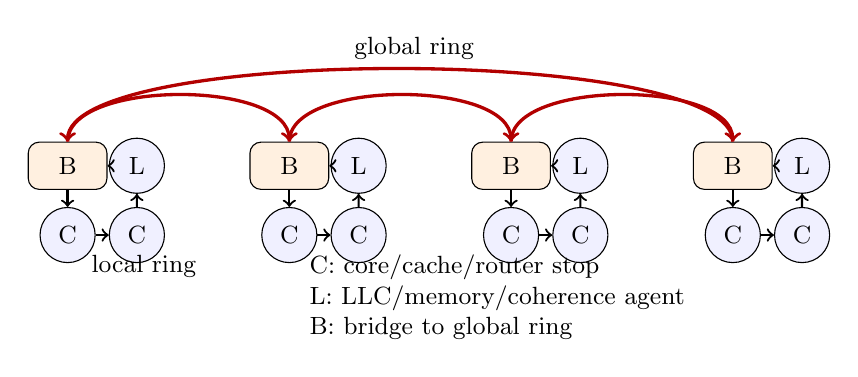
\begin{tikzpicture}[scale=0.88, every node/.style={font=\small}]
  \tikzstyle{rnode}=[circle,draw,minimum size=7mm,inner sep=1pt,fill=blue!6]
  \tikzstyle{bridge}=[rectangle,draw,rounded corners,minimum width=10mm,minimum height=6mm,fill=orange!12]
  \foreach \x/\name in {0/A,1/B,2/C,3/D} {
    \begin{scope}[shift={(\x*3.2,0)}]
      \node[rnode] (n1\x) at (0,0) {C};
      \node[rnode] (n2\x) at (1,0) {C};
      \node[rnode] (n3\x) at (1,1) {L};
      \node[bridge] (br\x) at (0,1) {B};
      \draw[->,thick] (n1\x) -- (n2\x);
      \draw[->,thick] (n2\x) -- (n3\x);
      \draw[->,thick] (n3\x) -- (br\x);
      \draw[->,thick] (br\x) -- (n1\x);
    \end{scope}
  }
  \draw[->,very thick,red!70!black] (br0.north) .. controls +(0,0.9) and +(0,0.9) .. (br1.north);
  \draw[->,very thick,red!70!black] (br1.north) .. controls +(0,0.9) and +(0,0.9) .. (br2.north);
  \draw[->,very thick,red!70!black] (br2.north) .. controls +(0,0.9) and +(0,0.9) .. (br3.north);
  \draw[->,very thick,red!70!black] (br3.north) .. controls +(0,1.4) and +(0,1.4) .. (br0.north);
  \node at (5.0,2.7) {global ring};
  \node at (1.1,-0.45) {local ring};
  \node[align=left] at (6.2,-0.9) {C: core/cache/router stop\\L: LLC/memory/coherence agent\\B: bridge to global ring};
\end{tikzpicture}
\caption{Simplified hierarchical-ring NoC. Local rings provide cheap nearby communication; bridge nodes transfer packets to a global ring. Deflection-based designs keep packets moving when ejection or bridge transfer is unavailable.}
\label{fig:hird}
\end{figure}

\section{Case study: Hierarchical Rings with Deflection Routing (HiRD)}

Ausavarungnirun et al.'s HiRD paper is a useful focal point because it combines three ideas that are individually old but jointly compelling for manycore CMPs: hierarchy, rings, and deflection routing \cite{Ausavarungnirun2014HiRD}.

\subsection{Topology motivation}

A flat ring is elegant at small scale, but the average traversal distance and bisection bottleneck grow with node count. A mesh improves bisection and distance but uses more complex routers, multi-port allocators, and often VCs. A hierarchical ring tries to land between them:

\begin{itemize}
  \item group nearby cores/cache slices on small local rings;
  \item connect those local rings through bridge routers to a global ring;
  \item keep local traffic local when possible;
  \item use the global ring only for inter-cluster traffic.
\end{itemize}

This is a topology-level answer to physical design: ring wires can be simple and predictable, local communication remains cheap, and global traffic no longer circles every node in the chip.

\subsection{Flow-control mechanism}

The flow-control problem in a hierarchical ring is concentrated at two places: ejection points and local/global bridge points. If a packet reaches its destination but the destination cannot accept it, a buffered design must stop or store it. If many packets want the bridge, a buffered design needs bridge queues and backpressure. HiRD's philosophy is to avoid much of that storage by allowing packets to continue around the ring and try again later. In other words, the ring itself becomes a circulating holding structure.

Conceptually:

\begin{enumerate}
  \item A packet on a local ring either ejects locally, transfers to a bridge/global ring if needed, or continues circulating.
  \item A packet on the global ring transfers to the destination local ring when a bridge opportunity is available; otherwise it continues around the global ring.
  \item Ejection and transfer must be prioritized over new injection often enough that in-flight packets make progress.
  \item Injection control prevents newly injected packets from consuming all opportunities and starving deflected packets.
\end{enumerate}

This is not ``flow control disappears.'' Rather, it moves from per-hop buffer credits to admission, ejection, and bridge-transfer policy. The design avoids global backpressure, but the designer still needs progress guarantees.

\subsection{Why deflection fits rings particularly well}

Deflection in a mesh can send packets onto non-minimal paths with many possible wrong turns. In a ring, the non-minimal path is often just another lap. That makes the mechanism simple: no complex output selection, and no large VC allocator. The cost is predictable too: extra laps consume ring bandwidth and increase latency variance.

For workloads with locality, local rings reduce pressure on the global ring, so deflection is relatively rare. For adversarial or all-to-all traffic, deflection becomes much more expensive because the global ring and bridge points become bottlenecks. This is the fundamental ring trade-off: cheap routers and wires, but hot bridges can dominate.

\subsection{Comparison against bubble/credit rings}

Bubble flow control and credit rings prevent overflow by stopping injection or forwarding. HiRD-style deflection prevents overflow by refusing to stop in-flight traffic. The distinction matters:

\begin{itemize}
  \item \term{Credit/bubble}: lower path inflation, but stalls can propagate around cycles; requires buffer accounting and may reduce usable capacity to preserve bubbles.
  \item \term{Deflection}: simpler transit path and fewer buffers, but uses extra bandwidth under contention; requires fairness and injection throttling rather than downstream credits.
  \item \term{VC ring}: more robust for multiple traffic classes and strict deadlock isolation, but loses much of the tiny-router advantage that made rings appealing.
\end{itemize}

\section{State of the art outside rings}

Because ring-specific work is narrower than mesh/torus NoC work, a credible survey must include broader NoC flow control. The mechanisms below define the practical design space.

\subsection{Credit-based wormhole with a few VCs}

This is the workhorse design point. Packets are flitized; routers use small input buffers; credits provide lossless local backpressure; VCs separate protocol classes and avoid routing/protocol deadlock. It is neither the lowest-buffer nor the lowest-latency design, but it is robust.

The reason it persists is not nostalgia. Cache-coherent multicore fabrics have request, response, data, snoop/probe, and sometimes retry/ack classes. Even if the routing topology is deadlock-free, the coherence protocol can create dependency cycles: a request may require a response, a response may require data-buffer availability, and probes can block unrelated traffic. Separate virtual networks or physically separate channels break these cycles. Arm CHI, for example, exposes separate REQ/RSP/SNP/DAT channels and L-credit flow control at the link layer \cite{ArmCHI2021}.

\subsection{Adaptive routing and escape resources}

Adaptive routing helps with nonuniform traffic, but it complicates deadlock freedom. Turn-model routing forbids selected turns to break cycles \cite{GlassNi1994,Chiu2000}. Duato's theory generalizes the design rule: adaptive channels can be used if there is a connected deadlock-free escape subnetwork and dependencies are constrained appropriately \cite{Duato1993}. In a NoC this often means one deterministic escape VC plus one or more adaptive VCs.

Regional congestion awareness and DyAD-style designs show how congestion signals can guide routing \cite{HuMarculescu2004,Gratz2008RCA}. The caveat is verification: adaptive routing can introduce reordering, starvation, QoS interference, and corner-case protocol interactions.

\subsection{Bypass: EVC and SMART}

Express virtual channels and SMART both attack per-hop router latency. EVCs provide multi-hop logical channels that bypass intermediate buffering/arbitration \cite{Kumar2007EVC}. SMART performs setup and then allows single-cycle multi-hop traversal across repeated links when resources are free \cite{Krishna2013SMART}. These mechanisms are attractive for low-load latency and diameter-heavy topologies, but harder to time and arbitrate than conventional one-hop-per-cycle routers. They are also less helpful at saturation, where contention rather than router pipeline latency dominates.

\subsection{Elastic, bufferless, and minimally buffered NoCs}

Buffers consume area, leakage, and allocator complexity. Elastic-buffer flow control stores flits in pipeline registers along links, reducing router input buffering \cite{Michelogiannakis2009Elastic}. Bufferless deflection removes most buffers and always forwards flits, misrouting some under contention \cite{Moscibroda2009,Fallin2011CHIPPER}. MinBD adds a small side buffer to recover much of the performance loss while retaining energy benefits \cite{Fallin2012MinBD}. Clumsy flow control is another attempt to raise throughput in bufferless NoCs without returning to full VC buffering \cite{Kim2013Clumsy}.

The mechanism-level lesson is close to HiRD: when you remove buffers, the network itself becomes the queue. This can be elegant at low to moderate load, but dynamic energy and tail latency can rise because packets travel extra hops.

\section{Industry signals}

Public industry documentation rarely reveals exact VC counts, credit pipelines, allocator policies, or deadlock proofs. Still, several sources are useful.

\subsection{Ring-based processors}

\term{Intel Sandy Bridge-era rings.} Public descriptions of Sandy Bridge report a coherent ring interconnect connecting cores, LLC slices, graphics, and the system agent, with separate request, snoop, acknowledge, and data rings \cite{Kanter2010Sandy}. The key flow-control implication is traffic-class separation: Intel exposed separate physical rings for coherence classes rather than a single undifferentiated packet stream. Exact credit and arbitration internals are not public.

\term{IBM Cell EIB.} Cell's EIB is a stronger public flow-control example: four data rings plus a command bus, pipelined circuit-switched transport, and end-to-end command credits for outstanding requests \cite{Ainsworth2006Cell}. It shows that commercial ring fabrics often prefer scheduled or credit-controlled transfer over fully general wormhole routing.

\subsection{Mesh and coherent-fabric processors}

\term{Tilera TILE64 iMesh.} TILE64 used five independent 2D mesh networks, each specialized for different traffic. Wentzlaff et al. describe three-entry credit-based flow control on tile-to-tile boundaries and separate physical networks for isolation, flow control, prioritization, and deadlock avoidance \cite{Wentzlaff2007Tilera}. This is one of the clearest public processor NoC sources linking topology, credits, and protocol deadlock.

\term{Arm CHI and CMN.} Arm CHI is a coherent interconnect protocol rather than a single topology. It defines protocol channels and L-credit flow control, and requires the network layer to support deadlock-free switching \cite{ArmCHI2021}. Linux kernel documentation describes CMN-600 as a configurable rectangular mesh of crosspoints with CHI agents \cite{LinuxCMN2023}. Together these are strong evidence for the industry pattern: channelized coherent traffic plus credit-controlled links over a mesh-like fabric.

\term{Intel Xeon Scalable and Xeon Phi.} Intel's public mesh white paper describes the move from rings to a 2D mesh with distributed cores, LLC slices, CHAs, snoop filters, memory controllers, and UPI agents \cite{IntelMesh2017}. Knights Landing similarly used a tiled 2D mesh with distributed tag directories \cite{Sodani2015KNL}. Public sources confirm topology and coherent-agent organization, but not router-level flow control.

\section{Design implications for a ring or hierarchical-ring NoC}

If the target topology resembles HiRD, the most important decisions are not just ``ring or mesh,'' but which congestion response is acceptable.

\subsection{When a ring is a good fit}

A ring or hierarchical ring is attractive when:

\begin{itemize}
  \item most traffic is local or can be clustered naturally;
  \item router area and verification simplicity are more important than peak bisection bandwidth;
  \item the floorplan benefits from predictable unidirectional or bidirectional channels;
  \item coherence traffic classes can be separated by physical rings, VCs, or carefully designed virtual networks;
  \item worst-case all-to-all traffic is not the dominant regime.
\end{itemize}

\subsection{Flow-control options for a modern hierarchical ring}

\begin{enumerate}
  \item \term{Conservative baseline: credit/bubble local rings plus separated traffic classes.} This is easiest to reason about. Use credits or ready/valid between ring stops, preserve bubbles on cyclic resources, and separate request/response/data/probe classes either physically or virtually. Good for correctness and bounded behavior; less elegant under long cyclic backpressure.
  \item \term{HiRD-like deflection: buffer-light local/global rings.} Use ejection-first arbitration, bridge-transfer priority over injection, and age or injection-throttling rules to guarantee progress. This minimizes buffering and avoids global stalls. It is best when extra laps are rare; it needs careful tail-latency evaluation.
  \item \term{Hybrid minimally buffered deflection.} Add tiny side buffers at bridge/ejection hot spots. This borrows from MinBD: a small amount of buffering can remove many harmful deflections while keeping the router simpler than a full VC design \cite{Fallin2012MinBD}. For a hierarchical ring, bridge nodes are the obvious place to spend the buffer budget.
  \item \term{VC-enhanced ring for coherence-heavy systems.} If strict message-class isolation is non-negotiable, add VCs or physically separate rings. This sacrifices some simplicity but aligns with industrial coherent-fabric practice.
\end{enumerate}

\subsection{What to measure}

A ring-flow-control evaluation should not stop at average latency. The key metrics are:

\begin{itemize}
  \item zero-load latency and saturation throughput;
  \item 95th/99th percentile latency under bursty and adversarial traffic;
  \item bridge utilization and deflection rate per bridge;
  \item injection stall rate or injection throttle duty cycle;
  \item number of extra laps per delivered packet;
  \item energy per delivered flit, including wasted deflection traversal;
  \item fairness across nodes, especially nodes near/away from bridges;
  \item protocol deadlock freedom with request, response, data, and snoop/probe classes.
\end{itemize}

For your topology interest, the hidden boss fight is bridge congestion. A hierarchical ring can look excellent under local traffic but collapse into a global-ring/bridge bottleneck under permutation, hotspot, or coherence-snoop-heavy traffic.

\section{Open problems and current research directions}

\begin{itemize}
  \item \term{Tail latency in bufferless rings.} Deflection papers often report average behavior and throughput, but production coherent fabrics care about outliers. Age-based priority and throttling help but can reduce injection bandwidth.
  \item \term{Protocol-aware flow control.} Many academic NoC evaluations use synthetic traffic or simplified cache-coherence models. Real request/response/probe/data dependencies can dominate correctness and sizing.
  \item \term{Hybrid buffering at structural bottlenecks.} Full buffering everywhere is expensive; no buffering anywhere is fragile. Hierarchical rings strongly suggest asymmetric buffering: spend queues at bridges, memory controllers, and ejection hotspots.
  \item \term{Physical-design co-optimization.} Rings are attractive partly because wires are predictable. SMART/EVC-like bypass and high-radix designs may win architecturally but lose timing/area battles at physical implementation.
  \item \term{QoS and isolation.} Heterogeneous multicore/accelerator SoCs need bandwidth/latency isolation. Token or slot rings have natural scheduling hooks; deflection designs need explicit admission and priority mechanisms.
\end{itemize}

\section{Bottom-line recommendation}

For a ring-based NoC study, I would treat the state of the art as a three-way comparison:

\begin{enumerate}
  \item \term{Credit/bubble hierarchical ring}: robust baseline, easier proof, moderate buffering.
  \item \term{HiRD-like deflection hierarchical ring}: buffer-light, simple routers, no global backpressure, but sensitive to bridge contention and tail latency.
  \item \term{Hybrid minimally buffered deflection ring}: likely best research direction if the objective is a practical modern ring. Add small buffers only at high-leverage points and use deflection as the fallback rather than the only congestion response.
\end{enumerate}

Against mesh NoCs, the ring design should be judged not only by throughput, but by router simplicity, floorplan compatibility, energy per delivered flit, and coherence verification cost. If all-to-all or many-to-memory traffic dominates, a mesh or hierarchical mesh with credit-based VC flow control is probably safer. If locality is strong and wire/router simplicity is paramount, hierarchical rings with carefully engineered deflection remain a credible design point.

\bibliographystyle{unsrtnat}
\bibliography{refs}

\end{document}
